  \documentclass[bulg]{beamer}
  \usetheme[NoLogo, MathSerif, latinmodern, neohellenic]{FzF}

  % LANGUAGE %
  \usepackage[T2A]{fontenc}
  \usepackage[utf8]{inputenc} 
  \usepackage[english, bulgarian]{babel}          % Automatic translations
  \usepackage{csquotes}       % Quotation marks
  \usepackage{microtype}      % Improved typography
  \usepackage{amssymb}        % Mathematical symbols
  \usepackage{dsfont}         % More math fonts
  \usepackage{mathtools}      % Mathematical symbols
  \usepackage[absolute, overlay]{textpos} % Arbitrary placement
  \setlength{\TPHorizModule}{\paperwidth} % Textpos units
  \setlength{\TPVertModule}{\paperheight} % Textpos units
  \usepackage{tikz, tikz-cd}
  \usetikzlibrary{overlay-beamer-styles}  % Overlay effects for TikZ
  \usepackage{booktabs}

  \def\department{Катедра „Теоретична Физика“}
  \def\faculty{Физически Факултет}

  \author{Иво Николаев Илиев}
  \title{Точни решения в холографски модели}
  \subtitle{Предзащита на дисертационен труд за придобиване на ОНС „Доктор“}
  \begin{document}

  % Use
  %
  %     \begin{frame}[allowframebreaks]{Title}
  %
  % if the TOC does not fit one frame.
  \begin{frame}{Съдържание}
      \tableofcontents
  \end{frame}


  \section{Струнна теория и AdS/CFT съответствие}
  \SectionPage
%%%%%%%%%%%%%%%%%%%%%%%% STRING THEORY SLIDE %%%%%%%%%%%%%%%%%%%%%%%%
  \subsection{Теория на струните - мотивация и действие}
  \begin{frame}
    \small
    \vspace{-0.2cm}
\begin{alertblock}{\small Теория на Струните}
 \centering
 Мирова линия (траектория) \implies \textit{мирова повърхнина}\\
 \vspace{10pt}
 \includegraphics[height = 2.5cm]{images/strings.png}
 \begin{equation*}
   \hspace{-1cm}S \propto \int\hspace{-0.5em}\underbrace{\strut\ \:d\ell\ \:}_{\text{дължина }}\quad\implies\quad S \propto\int\underbrace{\strut\ \: dA\ \:}_{\text{площ }}
   \end{equation*}
 \end{alertblock}%
\begin{exampleblock}{\small Действие на нелинеен сигма модел}
  \begin{equation*}    
        S_{\sigma}=\frac{1}{4\pi\alpha^{\prime}} \int_{\Sigma} d^{2} \xi    
        \sqrt{h}\left\{\left(h^{ab}G_{\mu\nu}(X)+\epsilon^{ab}B_{\mu
          \nu}(X)\right)    
        \partial_{a}X^{\mu}\partial_{b}X^{\nu}+\alpha^{\prime}R^{(2)}    
    \Phi(X)\right\}
    \end{equation*}
  \end{exampleblock}
\end{frame}
%%%%%%%%%%%%%%%%%%%%%%%% AdS CFT SLIDE 2 %%%%%%%%%%%%%%%%%%%%%%%%%%%%
  \begin{frame}
    \footnotesize
  \begin{figure}
    \includegraphics[width=0.75\textwidth]{images/adscft.png}
  \end{figure}
  \vspace{-0.5cm}
\begin{minipage}[t]{0.45\linewidth}%
  \begin{alertblock}{\footnotesize Граница на 'т Хофт и double scaling limit}
$\strut N \rightarrow \infty,\quad \lambda = 4\pi g_s N = \text{fixed}$
\end{alertblock}
\end{minipage}%
\hspace{1.35cm}
\begin{minipage}[t]{0.45\linewidth}%
  \begin{alertblock}{\footnotesize Съответствие на параметрите}
    $ \strut g_s \equiv  e^{\Phi} = g^2_{\textsc{YM}},\quad \ell^4 = \lambda \alpha^{\prime 2}$
\end{alertblock}
\end{minipage}
\begin{equation*}
  ds^2 = \left(1+\frac{\ell^4}{r^4}\right)^{-\frac{1}{2}}\eta_{ij}dx^i dx^j
  + \left(1+\frac{\ell^4}{r^4}\right)^{\frac{1}{2}}\left(dr^2+r^2
  d\Omega^2_5\right)
\end{equation*}
\begin{minipage}[t]{0.45\linewidth}%
  \begin{alertblock}{\footnotesize $r\gg \ell$ (далеч от набора брани)}
    $ds^2 = \eta_{ij} dx^i dx^j + dr^2 +r^2 d\Omega_5^2$
\end{alertblock}
\end{minipage}%
\hspace{1.35cm}
\begin{minipage}[t]{0.45\linewidth}%
  \begin{alertblock}{\footnotesize $r\ll\ell, z=\ell^2/r$ (в „гърлото“)}
      $ds^2 = \frac{\ell^2}{z^2}(\eta_{ij} dx^i dx^j +dz^2) + \ell^2
      d\Omega_5^2$
\end{alertblock}
\end{minipage}
\end{frame}

%%%%%%%%%%%%%%%%%%%%%%%% AdS/CFT SLIDE %%%%%%%%%%%%%%%%%%%%%%%%%%%%%%
\subsection{Холографско съответствие}
\begin{frame}
  \footnotesize
  \vspace{-0.4cm}
\begin{minipage}[t]{0.45\linewidth}%
\begin{table}[h]
  \toprule\\
  \\
  \begin{tabular}{c l c}
  \lambda \rightarrow \infty\ \quad\iff & \hspace{-0.3cm}$\ell^2 \gg \alpha^\prime$
                                          & \hspace{-1.9cm}$\rightarrow$ SUGRA\\
\\
\begin{tabular}{c c}
  & $\nearrow$\\
    крайно $\lambda$ & \\
  & $\searrow$
  \end{tabular}

                                          &\hspace{-0.6cm}

  \begin{tabular}{l}
    $N \rightarrow \infty$\\
    $g_s \rightarrow 0$\\
    \\
    \\
    произв.\\
    $N, g_{\textsc{YM}}$
  \end{tabular}

  &\hspace{-0.7cm}


  \begin{tabular}{l}
    $\rightarrow$ свободна\\ теория
    \\
    \\
    \\
    $\rightarrow$ теория\\
    с взаимодействия
  \end{tabular}
  \\
\end{tabular}
\\
\bottomrule
\end{table}
%%%%
%%%%
      \vspace{-0.3cm}
      \flushleft
      \begin{alertblock}{\footnotesize Съответствие}
        \footnotesize
        $Z_\text{SUGRA}(\phi^0_i) = \left\langle e^{\int d^4x \phi_i^0 \left\langle
          \mathcal{O}_i\right\rangle}\right\rangle_{\text{CFT}}$
    \end{alertblock}%
    \begin{exampleblock}{\footnotesize Скаларно поле в $AdS_{d+1}$}
      \footnotesize
    \begin{equation*}
      \footnotesize
      \phi(u,x)
      = \left(\frac{1}{u}\right)^{4-d}\hspace{-1em}\phi_0(x)+\left(\frac{1}{4}\right)^\Delta
      \hspace{-0.5em}\langle\mathcal{O}(x)\rangle
    \end{equation*}
    \begin{equation*}
      \Delta = \frac{d}{2} + \sqrt{\,\frac{d^4}{4} +\ell^2m^2}
    \end{equation*}
  \end{exampleblock}
    \end{minipage}%
    \begin{minipage}[t]{0.55\linewidth}
  \flushright
  \begin{align*}
  \phi(x,z) &\rightarrow \quad\mathcal{O}(x)\\
  A_{\mu}(x,z) &\rightarrow \quad J^\mu(x)\\
  g_{\mu\nu} &\rightarrow \quad T^{\mu\nu}(x)
\end{align*}
      \vspace{-0.5cm}
    \begin{figure}
      \flushright
      \includegraphics[width=0.9\textwidth]{images/drawing.png}
    \end{figure}
    \end{minipage}%
  \end{frame}

%%%%%%%%%%%%%%%%%%%%%%%% MAGNONS & SPIKES %%%%%%%%%%%%%%%%%%%%%%%%%%%
  \begin{frame}{}
  $AdS_5\times S^5$ -- граница на Пенроуз $\leftrightarrow$ Янг-Милс -- BMN граница 
  \begin{minipage}[t]{0.6\linewidth}%
  \begin{alertblock}{Дисперсионни съотношения в BMN границата}
  \item $E-J =0\implies$
  \begin{equation*}
    \mathcal{O} \sim \sum_q e^{iqp}\left(\ldots ZZZWZZZ\ldots\right)
  \end{equation*}
  \vspace{-0.5cm}
  \begin{gather*}
    J \rightarrow \infty,\;\lambda = \text{fixed},\; p = \text{fixed}
    \\
    \uparrow\downarrow\\
    \text{солитонно решение}
  \end{gather*}
\end{alertblock}
  $\lambda\gg 1$
  \begin{equation*}
    E-J=\frac{\sqrt{\lambda}}{\pi}\left|\sin \left(\frac{p_{\textsc{ws}}}{2}\right)\right|
  \end{equation*}
\end{minipage}%
  \begin{minipage}[t]{.4\textwidth}
    \vspace{0.2cm}
    \flushright
    \flushbottom
  \begin{figure}
      \centering
      \includegraphics[width=0.4\linewidth]{./images/magnon.pdf}
      \caption{Гигантски магнон}
      \label{figure1}
  \end{figure}
  \begin{figure}
      \centering
      \includegraphics[width=0.4\linewidth]{./images/spike.png}
      \caption{Шиповидна струна}
      \label{figure2}
  \end{figure}
  \end{minipage}%
  \end{frame}
%%%%%%%%%%%%%%%%%%%%%%%%%%%%%%%%%%%%%%%%%%%%%%%%%%%%%%%%%%%%%%%%%%%%%
  \section{Въведение в проблематиката}
  \SectionPage
  \subsection{Нерелативистка холография}
  \subsection{TsT трансформация}
  \subsection{Многообразия на Сасаки-Айнщайн, $T^{1,1}$}
%%%%%%%%%%%%%%%%%%%%%%%% MOTIVATION  SLIDE %%%%%%%%%%%%%%%%%%%%%%%%%%
  \begin{frame}
      \Huge
      \tikz[baseline,remember picture]{\node[rectangle, ultra thick,
      draw=bostonuniversityred,
    fill=structure!40,anchor=baseanchor=base](t1){{\strut AdS/CFT} };}
    \flushright
    \vspace{-1.8cm}
    \tikz[baseline,remember picture]{\node[rectangle, ultra thick,
    draw=bostonuniversityred,
    fill=bostonuniversityred!40,anchor=baseanchor=base](t2){{\strut Schrod/dipole-CFT} };}
    \normalsize
    \vspace{0.5cm}
    \begin{alertblock}{Деформация на хиперболичното пространство}
    \begin{align*}
    &\overset{\text{AdS}}{\text{Конформна Алгебра}}
    \overset{\text{нерелативистка
    граница*}}{\longrightarrow} \overset{\text{Schrod}}{\text{Алгебра на Шрьодингер}}
      \end{align*}
    \end{alertblock}
    \begin{alertblock}{Деформация на компактното пространство}
      \Large %
    \begin{align*}
      \underbrace{\strut\ \ \ S^5\ \ \ }_{\mathcal{N}=4}
      \overset{\text{\strut\tiny деформация}}{\longrightarrow} \underbrace{\strut\ \ T^{1,1}\ \ }_{\mathcal{N}=1}
      \end{align*}
    \end{alertblock}
    \begin{tikzpicture}[remember picture,overlay]   %% use here too
      \path[draw=structure,ultra thick,->,above,font=\footnotesize] (t1.east) to (t2.west);
    \end{tikzpicture}
  \end{frame}
%%%%%%%%%%%%%%%%%%%%%%%% SCHROD ALGEBRA %%%%%%%%%%%%%%%%%%%%%%%%%%%%% 
  \begin{frame}{}
  \begin{alertblock}{\small{Алгебра на Шрьодингер}}
  \begin{equation*}
    \begin{aligned}
      &\left[M_{ij},N\right] = \left[M_{ij}, D\right] =0, && \left[P_i,P_j\right] = \left[K_i, K_j\right] = 0, \\
      &\left[M_{ij}, P_k\right] = i(\delta_{ik}P_j - \delta_{jk}P_i), && \left[K_i,P_j\right] = i\delta_{ij}N,\\
      &\left[M_{ij}, K_k\right] = i(\delta_{ik}K_j - \delta_{jk}K_i), && \left[D, K_i\right] = -i K_i,\\
      &\left[M_{ij}, M_{kl}\right] = i(\delta_{ij}M_{jk} - \delta_{jk}M_{il}
      + \delta_{il}M_{kj} -\delta_{jl}M_{ki}), && \left[D, H\right] = 2iH,\\
      \end{aligned}
      \end{equation*}
      \begin{align*}
      &\left[H, N\right] = \left[H,P_i\right] = \left[H, M_{ij}\right]=0,\\
      &\left[H, K_i\right] = -i P_i,\\
      &\left[D, N\right] = 0.
  \end{align*}
  \end{alertblock}
  \tiny{
  Легенда:
  \begin{itemize}
      \item $M_{ij}$ са генераторите на пространствени въртения.
      \item $P_i$ са импулсите.
      \item $K_i$ са бустове на \emph{Галилей}.
      \item $N$ е броят частици
      \item $D$ е операторът на дилатации
  \end{itemize}}
  \end{frame}
%%%%%%%%%%%%%%%%%%%%%%%% SCHR_5 x S^5 %%%%%%%%%%%%%%%%%%%%%%%%%%%%%%%
  \begin{frame}{}
  \begin{alertblock}{Метрика за $Schr_5\times S^5$}
      \vspace{-0.2cm}
  \begin{equation*}
    \frac{ds^2}{\ell^2} = -\left(1+\frac{\mu^2}{Z^4} - \frac{X_1^2+X_2^2}{Z^2}\right)d T^2
    + \frac{1}{Z^2}\left(2d
    Td V + d X_1^2 + d X_2^2 + d Z^2\right) + d s^2_{\mathbb{S}^5}
  ,
  \end{equation*}
  \end{alertblock}

  \begin{minipage}[t]{0.5\linewidth}%
    \begin{exampleblock}{Сферична част}
      \vspace{-0.5cm}
    \begin{equation*}
      ds^2_{\mathbb{S}^5} = d\theta^2 + \cos^2\theta d\psi^2
      + \sin^2\theta d\Omega^2_3
    \end{equation*}
    \begin{equation*}
     d \Omega^2_3 = d \eta^2 + \sin^2\eta d \varphi_1^2 + \cos^2\eta d\varphi^2_2
    \end{equation*}
    \end{exampleblock}
  \end{minipage}%
  \begin{minipage}[t]{0.5\linewidth}%
  \vspace{0.25cm}
  \begin{itemize}
    \item \alert{TsT} трансформация:
      \begin{enumerate}
        \item \alert{T}-дуалност по изометрично направление,
        \item транслация (\alert{s}hift) с параметър $\mu$
        \item \alert{T}-дуалност обратно началното направление.
      \end{enumerate}
  \end{itemize}
  \end{minipage}%
  \begin{equation*}
    S \supset \mathcal{M}\sim T^2 = (S^1\times S^1) (\phi_1,\phi_2)
  \end{equation*}
  \vspace{-0.5cm}
  \begin{alertblock}{TsT за AdS}
  \begin{equation*}
    AdS_5\times S_5 \xrightarrow{\text{TsT}} Schr_5\times S_5\ (+\ \text{
    $B$ поле})
  \end{equation*}
  \end{alertblock}
  \end{frame}
%%%%%%%%%%%%%%%%%%%%%%%% SASAKI MANIFOLDS %%%%%%%%%%%%%%%%%%%%%%%%%%%
  \begin{frame}
    \begin{definition}[Многообразие на Сасаки]
      Нека $(S,g)$ е риманово многообразие и
        \begin{equation*}
          C(S,g) = \mathds{R}_{>0}\times S,\quad g_C =dr^2 + r^2g.
        \end{equation*}
        Тогава
        $(S,g)$ е Сасаки $\iff C(S,g)\text{ е келерово многообразие}$.
    \end{definition}%

    \begin{definition}[Многообразие нa Айнщайн]
      $(S,g)$ е многообразие на Айнщайн $\iff g_{ij} = \lambda R_{ij}$.
    \end{definition}%

    \begin{examples}
      \begin{align*}
        S^{2n-1}&\overset{C(S,g)}{\rightrightarrows}\mathbb{C}^{n}\backslash\left\{0\right\}\\
        T^{1,1}&\overset{C(S,g)}{\rightrightarrows} \text{конично многообразие
         (conifold)}
      \end{align*}
    \end{examples}
  \end{frame}
%%%%%%%%%%%%%%%%%%%%%%%%%%%%% T^{1,1} SLIDE %%%%%%%%%%%%%%%%%%%%%%%
  \begin{frame}
    \begin{minipage}[t]{0.3\linewidth}
      \Huge
      \vspace{2cm}
      \tikz[baseline,remember picture]{\node[rectangle, ultra thick,
      draw=bostonuniversityred, fill=bostonuniversityred!20,anchor=baseanchor=base](t1){{$T^{1,1}$} };}
    \end{minipage}%
    \begin{minipage}[t]{0.7\linewidth}
    \begin{alertblock}{Фактор-пространство}
    \begin{equation*}
      \tikz[remember picture] \node[coordinate] (n1) {};
      \frac{SU(2)\times SU(2)}{U(1)}\implies\text{топология на тор}
    \end{equation*}
    \end{alertblock}
    \begin{alertblock}{Метрика}
    \begin{multline*}
      \tikz[remember picture] \node[coordinate] (n2) {};
      ds^2_{T^{1,1}} = \frac{1}{6}\left(d\theta^2_1+\sin^2\theta_1
      d\phi^2_1\right) +\frac{1}{6}\left(d\theta_2^2 + \sin^2\theta_2 d\phi_2^2\right)
      \\+ \frac{1}{9} {\left(d\psi + \cos\theta_1 d\phi_1 + \cos\theta_2
      d\phi_2\right)}^2,\quad (\theta,\phi) \in S^3,\psi \in U(1)
    \end{multline*}
    \end{alertblock}
    \end{minipage}%
    \vspace{0.5cm}
  Оказва се, че $C(S,g)$ допуска 2 реални килингови спинора - $\mathcal{N}=1$
    суперсиметрия
    \begin{tikzpicture}[remember picture,overlay]   %% use here too
      \path[draw=structure,ultra thick,->] (t1.east) to ([yshift=1mm,xshift=-19mm]n1);
      \path[draw=structure,ultra thick,->] (t1.east) to ([yshift=2mm,xshift=-5mm]n2);
    \end{tikzpicture}
  \end{frame}
%%%%%%%%%%%%%%%%%%%%%%%% CONIFOLD SETUP %%%%%%%%%%%%%%%%%%%%%%%%%%%%%
  \begin{frame}
    \vspace{-1em}
    \begin{alertblock}{Същина на изследваната геометрична конфигурация}
    \begin{equation*}
        \mathds{M}_4 \times \text{Конифолд} \rightarrow \text{Hyp(AdS/Schr)}_5
      \times \text{Сасаки-Айнщайн}^5 
    \end{equation*}
\begin{equation*}
  -dt^2 +d\vec{x}^2 + dr^2+r^2g_5 \rightarrow \frac{1}{r^2}(-dt^2 + dr^2
  + d\vec{x}^2) + g_5
\end{equation*}

    \begin{figure}
      \includegraphics[width=0.55\textwidth]{images/ads4x6.png}
    \end{figure}
  \end{alertblock}
  \end{frame}
%%%%%%%%%%%%%%%%%%%%%%%% SUMMATION %%%%%%%%%%%%%%%%%%%%%%%%%%%%%%%%%%
  \begin{frame}
    \begin{alertblock}{Мотивация и задачи}
    \begin{itemize}
      \item \alert{Мотивация:}  Солитонни решения $\iff$ оператори (спин верижки).
      \item \alert{Обща задача:} Обобщаване на съответствието до нерелативистката му версия
        - Schrod/dipole-CFT.
      \item \alert{Конкретна задача:} Намаляване на симетрията разглеждайки
        $T^{1,1}$ като компактна част.
    \end{itemize}
  \end{alertblock}
  \begin{alertblock}{Какво следва}
    \begin{itemize}
      \item Изследване на нелинеен струнен сигма модел върху $Schr_5\times
        T^{1,1}$.
      \item Налагане на определен струнен анзац; определяне на параметрите
        задаващи профилите на струнните солитонни решения.
      \item Определяне на дисперсионните съотношения и сравнения с известни
        резултати за по-симетрични случаи.
    \end{itemize}
  \end{alertblock}
  \end{frame}
%%%%%%%%%%%%%%%%%%%%%%%%%%%%%%%%%%%%%%%%%%%%%%%%%%%%%%%%%%%%%%%%%%%%%
  \section{Изследване на струнни решения върху $Schr_5\times T^{1,1}$}
  %
  \SectionPage
  \subsection{Постановка на задачата}
  \subsection{Анзац за решенията, уравнения за движение}
  \subsection{Параметри на солитонното решение}
  \subsection{Дисперсионни съотношения}
%%%%%%%%%%%%%%%%%%%%%%%% SCHROD x T11 %%%%%%%%%%%%%%%%%%%%%%%%%%%%%%%
  \begin{frame}{}
    \begin{alertblock}{Действие}
      \vspace{-0.2cm}
  \begin{align*}
    S=\int d \tau d \xi L&=-\frac{T}{2 \alpha} \int d \tau d \xi \left\{G_{M N}\left[-\partial_{\tau} X^{M} \partial_{\tau} X^{N}-2 \beta \partial_{\tau} X^{M} \partial_{\xi} X^{N}\right.\right.\\
   &\left.\left.+\left(\alpha^{2}-\beta^{2}\right) \partial_{\xi} X^{M}
   \partial_{\xi} X^{N}\right]+2 \alpha B_{M N} \partial_{\tau} X^{M}
 \partial_{\xi} X^{N}\right\},
 \alert{\xi = -\alpha\sigma + \beta\tau}
  \end{align*}
  \end{alertblock}
  \begin{exampleblock}{Метрика и $B$-поле}
    \small
  \begin{equation*}
  ds^2_{Schr_{5} \times T^{1,1}}=d s_{S c h r_{5}}^{2}+d s_{T^{1,1}}^{2}
  \end{equation*}

  \begin{equation*}
  d s_{T^{1,1}}^{2}=\frac{b}{4}\left[\sum_{i=1}^{2}\left(d \theta_{i}^{2}+\sin
  ^{2} \theta_{i} d \phi_{i}^{2}\right)+b\left(d \psi-\sum_{i=1}^{2} \cos
  \theta_{i} d \phi_{i}\right)^{2}\right]
  \end{equation*}

\begin{equation*}
  B_{(2)} = \frac{b\mu}{2Z^2}dT \wedge \left(d\psi - \sum_{i=1}^2 \cos\theta_i
  d\phi_i\right)
\end{equation*}
\end{exampleblock}
\end{frame}
%%%%%%%%%%%%%%%%%%%%%%%% ANZATZ %%%%%%%%%%%%%%%%%%%%%%%%%%%%%%%%%%%%%
\begin{frame}
\begin{alertblock}{Връзки на Вирасоро}%
  \vspace{-0.5cm}
\begin{align*}
\operatorname{Vir}_{1}:\  & G_{M N}\left(\partial_{\tau} X^{M} \partial_{\tau} X^{N}+2 \beta \partial_{\tau} X^{M} \partial_{\xi} X^{N}+\left(\alpha^{2}+\beta^{2}\right) \partial_{\xi} X^{M} \partial_{\xi} X^{N}\right)=0 \\
\operatorname{Vir}_{2}:\  & G_{M N}\left(\partial_{\tau} X^{M} \partial_{\xi} X^{N}+\beta \partial_{\xi} X^{M} \partial_{\xi} X^{N}\right)=0
\end{align*}
\end{alertblock}
\alert{Анзац} за решенията 
\begin{align*}
&T=\kappa \tau+t(\xi), \kappa>0, \quad V=\omega_{0} \tau+v(\xi), \quad Z=c o n s t \neq 0, \quad \vec{X}=\overrightarrow{0} \\
&\theta_{i}=\theta_{i}(\xi), \quad \phi_{i}=\omega_{i} \tau+\Phi_{i}(\xi), \quad
i=1,2, \quad \psi=\omega_{3} \tau+\Psi(\xi),\\
\label{eq:ansatz}
\end{align*}
\alert{Твърд} профил, движещ се по геодезична върху компактното многообразие.
Изометрии - транслации по $T, V, \phi_1, \phi_2, \psi$
\begin{alertblock}{Импулси}
\begin{equation*}
\Pi_T = \frac{\partial L}{\partial \dot{T}}, \quad
\Pi_V = \frac{\partial L}{\partial \dot{V}}, \quad
\Pi_{\phi_k} = \frac{\partial L}{\partial \dot{\phi}k},\quad 
\Pi_{\psi} = \frac{\partial L}{\partial \dot{\psi}},\quad 
\end{equation*}
\end{alertblock}
\end{frame}
%%%%%%%%%%%%%%%%%%%%%%%% EQUATIONS %%%%%%%%%%%%%%%%%%%%%%%%%%%%%%%%%%
\begin{frame}
  Дефинираме $\mathcal{M}={Schr_5\times T^{1,1}}\Big\vert_{\theta_2,\phi_2
  = \text{fixed}} \rightarrow$ подсектор на теорията.
 
  \begin{alertblock}{Уравнение за движение ($\theta$)}
    \vspace{-0.5cm}
\begin{multline*}
\left(\alpha^{2}-\beta^{2}\right)^{2} \theta^{\prime 2}=-\sin ^{2} \theta\left\{\left(\alpha^{2}-\beta^{2}\right) \omega_{1}^{2}+\left[\frac{4 A}{b} \frac{(1+\cos \theta)}{\sin ^{2} \theta}+\beta \omega_{1}\right]^{2}\right\} \\
-\left(\alpha^{2}-\beta^{2}\right) b\left(\omega_{3}-\omega_{1} \cos \theta\right)^{2}-b\left[\beta\left(\omega_{3}-\omega_{1} \cos \theta\right)+\frac{4}{b^{2}}\left(A-\frac{\alpha b \mu \kappa}{2 Z^{2}}\right)\right]^{2} \\
-\left(\alpha^{2}-\beta^{2}\right) \frac{4}{b}\left(-\left|G_{T T}\right| \kappa^{2}+\frac{2 \omega_{0} \kappa}{Z^{2}}\right)
\label{eq:equiationfortheta}
\end{multline*}
\end{alertblock}
\begin{exampleblock}{Уравнения за движение + връзки на Вирасоро}
\begin{equation*}
  \theta(\xi) \implies v(\xi),\; \Phi(\xi),\; \Psi(\xi). \quad u(\xi) = \cos^2\frac{\theta(\xi)}{2}, u(\xi) \in \left[0,1\right]
\end{equation*}
\end{exampleblock}
\end{frame}


\begin{frame}
  \begin{alertblock}{Търсене на $u(\xi)$}
\begin{equation*}
  {u(\xi)^\prime}^2 = a_4 u^4 + a_3 u^3 + a_2 u^2 + a_1 u^1 + a_0 \equiv
  P_4(u),
  \label{eq:diffu2}
\end{equation*}
\begin{equation*}
a_0 = a_1 =0,
\end{equation*}
\begin{equation*}
  {u(\xi)^\prime}^2 = u^2(a_4 u^2 + a_3u + a_2)\equiv P_4(u)\geq 0
\quad P_4(u) \rightarrow  U(u).\\
  \label{eq:diffu}
\end{equation*}
\end{alertblock}

\begin{exampleblock}{Изразяване чрез константите от анзаца}
\tiny
\begin{equation*}
a_{4}=-\frac{4(1-b) \alpha^{2}
\omega_{1}^{2}}{\left(\alpha^{2}-\beta^{2}\right)^{2}}<0, \quad
  a_{3}=\frac{1}{(\alpha^2-\beta^2)^2}\left(4(1-b) \alpha^{2} \omega_{1}^{2}+4
    \alpha^{2} \omega_{1}^{2}-4 b \alpha^{2}
    \omega_{1}\left(\omega_{1}+\omega_{3}\right)+\frac{8 \alpha \beta \mu
  \kappa \omega_{1}}{Z^{2}}\right)
\end{equation*}
\begin{equation*}
  a_{2}=\frac{1}{(\alpha^2-\beta^2)^2}\left(-4 \alpha^{2} \omega_{1}^{2}+4
    b \alpha^{2} \omega_{1}\left(\omega_{1}+\omega_{3}\right)-\frac{8 \alpha
      \beta \mu \kappa \omega_{1}}{Z^{2}}-\frac{16
  A^{2}}{b^{2}}\right),\quad
  a_4 + a_3 + a_2 = -\frac{16 A^2}{b^2(\alpha^2-\beta^2)^2}
  \label{eq:polynomialandansatz}
\end{equation*}
\end{exampleblock}
  \begin{equation*}
    u(\xi)=\frac{2a_2}{B\cosh
    \left(\sqrt{a_{2}}\xi\right)-a_3},\quad B = \sqrt{a_{3}^{2}-4 a_{4}
  a_{2}},\quad a_2>0,\quad\frac{|a_3|}{B}<1
  \end{equation*}
\end{frame}



%%%%%%%%%%%%%%%%%%%%%%%% CONSTANTS RELATIONS %%%%%%%%%%%%%%%%%%%%%%%%
\begin{frame}
   \centering
    \begin{alertblock}{Алгебрични връзки за константите}
    \begin{align*}
        &Z^{2}\left(2\left(\beta^{2}-\alpha^{2}\right) \omega_{0}+\frac{4 \alpha \mu}{b}
           A+\alpha \beta b \mu\left(\omega_{1}+\omega_{3}\right)\right)=2 \beta^{2}
           \mu^{2} \kappa\\
        &\left(\omega_{1}+\omega_{3}\right)\left(A-\frac{\alpha b \mu}{2 Z^{2}}
          \kappa\right)=\beta\left(\frac{2 \omega_{0}}{Z^{2}} \kappa-\left|G_{T T}\right|
          \kappa^{2}\right)
      \end{align*}
    \end{alertblock}
    \vspace{-0.2cm}
\begin{exampleblock}{Струнни профили}
\begin{equation*}
\begin{aligned}
&\frac{4}{b^{2}}\left(A-\frac{b \alpha \mu}{2 Z^{2}}
  \kappa\right)=-\beta\left(\omega_{1}+\omega_{3}\right) \quad \text
  {гигантски магнони}\\
&\frac{4}{b^{2}}\left(A-\frac{b \alpha \mu}{2 Z^{2}}
\kappa\right)=-\frac{\alpha^{2}}{\beta}\left(\omega_{1}+\omega_{3}\right) \ 
\text{единични шиповидни струни}
\end{aligned}
\end{equation*}
\end{exampleblock}
\end{frame}
%%%%%%%%%%%%%%%%%%%%%%%% CONSTANTS FIXING %%%%%%%%%%%%%%%%%%%%%%%%%%%
\begin{frame}
\begin{minipage}[t]{0.45\linewidth}%
  \begin{alertblock}{\strut Магнони}
    \vspace{-0.5cm}
\begin{align*}
  A_{m}&=\frac{\alpha b}{2}\left[\frac{\omega_{0}}{\mu}-\frac{\beta b}{2
\alpha}\left(\omega_{1}+\omega_{3}\right)\right]\\
  \kappa_{m}^{2}&=\frac{\omega_{0}^{2}}{\mu^{2}}+\frac{b^{2}}{4}\left(\omega_{1}+\omega_{3}\right)^{2}\\
  Z_{m}^{2}&=\frac{\mu^{2} \kappa_{m}}{\omega_{0}} 
\end{align*}
\end{alertblock}
\end{minipage}%
\hspace{1cm}
\begin{minipage}[t]{0.45\linewidth}%
  \begin{alertblock}{\strut Шиповидни струни}
    \vspace{-0.5cm}
    \begin{align*}
      A_{s}&=\frac{\alpha b}{2} \frac{\omega_{0}}{\mu}\\
  \kappa_{s}^{2}&=\frac{\omega_{0}^{2}}{\mu^{2}}\\
  Z_{s}^{2}&=\frac{2 \beta \mu^{2} \kappa_{s}}{2 \beta \omega_{0}+b \mu
  \alpha\left(\omega_{1}+\omega_{3}\right)}
  \end{align*}
\end{alertblock}
\end{minipage}

\begin{multline*}
  \text{Aнзац + Уравнения за движение + Връзки на Вирасоро } \\ \implies 
      \tikz[baseline,remember picture]{\node[rectangle, ultra thick,
      draw=bostonuniversityred, fill=bostonuniversityred!20,anchor=baseanchor=base](t1){{$\text{
    Гигантски  магнони / (Единични) шиповидни струни върху } Schr_5\times
    T^{1,1}$} };}
\end{multline*}
\end{frame}
%%%%%%%%%%%%%%%%%%%%%%%% CALCULATIONS OF DISPERSSIONS %%%%%%%%%%%%%%%
\begin{frame}
  \tiny
  \begin{alertblock}{\tiny Плътности на импулси}
\vspace{-0.5cm}
\begin{align*}
  \frac{2 \alpha}{T} \Pi_{T} &=-2\Big(G_{T T}\left(\kappa+\beta
  t^{\prime}\right)+G_{T V}\left(\omega_{0}+\beta v^{\prime}\right)-\alpha
\sum_{i=1}^{2} B_{T \phi_{i}} \Phi_{i}^{\prime}-\alpha B_{T \psi}
\Psi^{\prime}\Big)\\
  \frac{2 \alpha}{T} \Pi_{V} &=2 G_{T V}\left(\kappa+\beta
      t^{\prime}\right)\\
  \frac{2 \alpha}{T} \Pi_{\phi_{k}} &=2\Big(\sum_{i=1}^{2} G_{\phi_{k}
        \phi_{i}}\left(\omega_{i}+\beta \Phi_{i}^{\prime}\right)+G_{\phi_{k}
    \psi}\left(\omega_{3}+\beta \Psi^{\prime}\right)+\alpha B_{T \phi_{k}}
  t^{\prime}\Big)\\
  \frac{2 \alpha}{T} \Pi_{\psi} &=2\Big(\sum_{i=1}^{2} G_{\phi_{i}
    \psi}\left(\omega_{i}+\beta \Phi_{i}^{\prime}\right)+G_{\psi
  \psi}\left(\omega_{3}+\beta \Psi^{\prime}\right)+\alpha B_{T \psi}
  t^{\prime}\Big)
      \end{align*}
    \end{alertblock}
  \small
\begin{exampleblock}{Сходяща комбинация}
 \begin{equation*}
    \Delta \equiv \frac{\Delta \phi + \Delta \psi}{2} = \int_{-\infty}^\infty d\xi
    \left (\frac{\Phi^\prime + \Psi^\prime}{2}\right)
  \end{equation*}
\end{exampleblock}
\begin{exampleblock}{Израз в явен вид}
\begin{equation*}
  \Delta=``\frac{1}{\left(\alpha^{2}-\beta^{2}\right)}\left\{\frac{1}{2}\left[\frac{4}{b^{2}}\left(A-\frac{b
  \alpha \mu}{2 Z^{2}}
  \kappa\right)+\beta\left(\omega_{1}+\omega_{3}\right)\right]\right\}
  \int_{-\infty}^{+\infty} d \xi\,\text{''} +\gamma
\end{equation*}
\end{exampleblock}
\end{frame}

%%%%%%%%%%%%%%%%%%%%%%%% NEW DISPERSSIONS RELATIONS %%%%%%%%%%%%%%%%%
\begin{frame}{}
  {\centering{\alert{Трансцендентни уравнения}}}
\begin{alertblock}{Дисперсионни съотношения - магнони}
  \tiny
  \vspace{-0.5cm}
  \begin{multline*}
\frac{\cos
\left\{\sqrt{\frac{(1-b)}{b^{2}}\left[\left(\frac{E}{T}\right)^{2}-\mu^{2}\left(\frac{J_{V}}{T}\right)^{2}\right]}-\frac{2
\sqrt{1-b}}{b^{2}}\left(\frac{J_{\psi}}{T}\right)\right\}-\cos \Delta}{\sin \left\{\sqrt{\frac{(1-b)}{b^{2}}\left[\left(\frac{E}{T}\right)^{2}-\mu^{2}\left(\frac{J_{V}}{T}\right)^{2}\right]}-\frac{2 \sqrt{1-b}}{b^{2}}\left(\frac{J_{\psi}}{T}\right)\right\}}= 
\sqrt{\frac{1}{2(1-b)}\left[\left(\frac{E}{T}\right)^{2}-\mu^{2}\left(\frac{J_{V}}{T}\right)^{2}\right]}-\frac{1}{b
\sqrt{1-b}}\left(\frac{J_{\phi}}{T}\right)
\label{eq:magnon}
\end{multline*}
\end{alertblock}
\vspace{0.2cm}
\begin{alertblock}{Дисперсионни съотношения - единична шиповидна струна}
\begin{equation*}
\frac{\cos \left[\frac{2 \sqrt{1-b}}{b^{2}}\left(\frac{J_{i j}}{T}\right)\right]-\cos \left\{\frac{1}{b}\left[\left(\frac{E}{T}\right)-\mu\left(\frac{J_{V}}{T}\right)\right]-\Delta\right\}}{\sin \left[\frac{2 \sqrt{1-b}}{b^{2}}\left(\frac{J_{\psi}}{T}\right)\right]}=\frac{1}{b \sqrt{1-b}}\left(\frac{J_{\phi}}{T}\right)
\end{equation*}
\end{alertblock}

\begin{minipage}[t]{0.6\textwidth}
  \vspace{-0.5cm}
  \begin{align*}
    b &\rightarrow 1 \implies Schr_5\times S^5 \;(\text{алгебрично})\\
    \mu &\rightarrow 0 \implies AdS_5\times T^{1,1} \;(\text{алгебрично})
  \end{align*}
\end{minipage}
\end{frame}
%%%%%%%%%%%%%%%%%%%%%%%% CONTRIBUTIONS %%%%%%%%%%%%%%%%%%%%%%%%%%%%%%

\begin{frame}
  \footnotesize
  \begin{alertblock}{\small Научни приноси}
    \begin{itemize}
      \item Решена е класическа струнна теория върху $Schr_5\times T^{1,1}$ на
        ниво уравнения за движение. Намерени са решения тип „гигантски
        магнони“ и „шиповидни струни“.
      \item Получени са явни изрази за дисперсионните съотношения,
        отговарящи на тези струнни конфигурации. Те са трансцендентни уравнения
        за аномалната размерност $\Delta$, за разлика от подобни структури върху
        по-симетрични пространства.
      \item Силно нетривиалните уравнения за аномалната размерност се нуждаят от
        аргументация. Тяхната валидност е проверена чрез налагане на
        съответните гранични преходи за параметрите на деформации. Получени са
        известните от литературата резултати.
    \end{itemize}
  \end{alertblock}


  \begin{alertblock}{\small Бъдещи изследвания}
    \begin{enumerate}
      \item Разглеждане на информационно-теоретичната страна на нерелативистката
        версия на холографската дуалност.
      \item Изследване на геометрични потоци върху многообразия на Шрьодингер.
        Интерес представлява геометричното изучаване на TsT трансформацията.
      \item Започната е работа по изследване на пространства на Шрьодингер,
        деформирани посредством оператора на Замолодчиков, $T\overline{T}$.
    \end{enumerate}
  \end{alertblock}
\end{frame}
%%%%%%%%%%%%%%%%%%%%%%%% PUBLICATIONS %%%%%%%%%%%%%%%%%%%%%%%%%%%%%%%
\begin{frame}
  \footnotesize
  \begin{alertblock}{\small{Публикации}}
  %A Golubtsova, H Dimov, \alert{I Iliev}, M Radomirov, RC Rashkov, T Vetsov,
  \textit{More on Schrödinger holography}. J. High Energ. Phys. 2020, 90
  (2020).\\

  %A Golubtsova, H Dimov, \alert{I Iliev}, M Radomirov, RC Rashkov, T Vetsov,
  Pulsating strings in $\text{Schr}_5\times T^{1,1}$ background. J. Phys. A:
  Math. Theor. 54 035401 (2020)\\

  Near-Flat Limit of $\text{Schr}_5 \times S^5$,
  Journal of Physics and Technology, Volume 3 (2019) Number 2
\end{alertblock}

\begin{exampleblock}{\small{В подготовка}}
    Geometric Flows for Holographic Backgrounds\\

    $T\overline{T}$ deformations and Schrödinger Backgrounds
  \end{exampleblock}
\end{frame}
\begin{frame}
  \begin{alertblock}{\small{Участие в конференции}}
  \footnotesize
    „Суперсиметрична локализация върху повърхности на Хопф“, Национална научна
    конференция по Физика, Пловдив, 2018 (постер)\\[15pt]
    „Near-flat Limit of $\text{Schr}_5\times S^5$, Национална научна
    конференция по Физика, Пловдив, 2019\\[15pt]
    „$T\overline{T}$ deformations and applications to non-relativistic holograhy“, 
    CERN-SEENET-MTP School „Computational Methods in Theoretical Physics“,
    24-27 Септември 2020, Крайова, Румъния\\[15pt]
    CERN-SEENET-MTP School ”High Energy and Particle Physics : Theory and
    Phenomenology”, 3-10 June 2018, Niˇs (Serbia).\\[15pt]
    CERN-SEENET-MTP School ”High Energy and Particle Physics : Theory and
    Phenomenology”, 3-9 June 2019, Ioannina (Greece).
  \end{alertblock}
\end{frame}

%%%%%%%%%%-----------------------------------------------------------%%%%%%%%%%%%%%%%%%%%
\end{document}
